
\documentclass[11pt,a4paper]{article}
\usepackage[hyperref]{fusionIR}
\usepackage{times}
\usepackage{latexsym}
\usepackage{fontspec}
\setmainfont{Lucida Grande} % Или другой шрифт, поддерживающий кириллицу
% \usepackage[T2A]{fontenc}
% \usepackage[utf8]{inputenc}
\usepackage[russian,english]{babel}
\def\Plus{\texttt{+}}
\def\Minus{\texttt{-}}
\renewcommand{\UrlFont}{\ttfamily\small}
\usepackage{times}
\usepackage{algorithm}
\usepackage{algpseudocode}
\usepackage{microtype}
\usepackage{minted}
\usepackage[a4paper, margin=0.5in]{geometry} % Поля страницы
\usepackage{etoolbox}
\usepackage{changepage}

% Отключение отступов для minted
\AtBeginEnvironment{minted}{\setlength{\parindent}{0pt}} 

\aclfinalcopy %


\usepackage{amsmath}
\usepackage{amssymb}
\usepackage{hyperref}
\usepackage{booktabs}
\usepackage{pgfplots}
\pgfplotsset{width=.9\columnwidth}
\usepackage{multirow}
\usepackage{caption}
\usepackage{subcaption}
\usepackage{tikz}
\usepackage{xspace}
\usepackage{xargs}
\usepackage[colorinlistoftodos,prependcaption,textsize=tiny]{todonotes}
\usepackage{multirow}
\usetikzlibrary{positioning}
\usepackage{pifont}
\newcommand{\cmark}{\text{\ding{51}}}
\newcommand{\xmark}{\text{\ding{55}}}
\usepackage{makecell}


\newcommand\BibTeX{B\textsc{ib}\TeX}
\newcommand\ignore[1]{}
\renewcommand{\UrlFont}{\ttfamily\small}

\def\model/{DPR}

\newcommand{\barlas}[1]{{\color{blue} [Barlas]: {#1}}}
\newcommand{\danqi}[1]{{\color{magenta} [Danqi: {#1}]}}
\newcommand{\scott}[1]{{\color{purple} [Scott: {#1}]}}
\newcommand{\vladk}[1]{{\color{red} [Vlad: {#1}]}}
\newcommand{\sergey}[1]{{\color{violet} [Sergey: {#1}]}}
\newcommand{\sewon}[1]{{\color{purple!50!orange} [Sewon: {#1}]}}



\newcommandx{\sy}[2][1=]{\todo[linecolor=purple,backgroundcolor=purple!10,bordercolor=purple,#1]{Scott: #2}\xspace}
\newcommandx{\dc}[2][1=]{\todo[linecolor=blue,backgroundcolor=blue!10,bordercolor=blue,#1]{Danqi: #2}\xspace}




\newcommand\sys[1]{\textsc{#1}}
\newcommand\ti[1]{\textit{#1}}
\newcommand\tf[1]{\textbf{#1}}
\newcommand\ttt[1]{\texttt{#1}}
\newcommand\mf[1]{\mathbf{#1}}

\newcommand*\samethanks[1][\value{footnote}]{\footnotemark[#1]}

\pgfplotsset{compat=1.14}

\title{Семантический поиск с дополнением контекстных ключевых слов через их объяснение}

\author{\makecell{Igor Tarlinskiy\thanks{\hspace{.06in}Equal contribution}, Elena Kreines, Sergey Glavatskii} \\
Moscow State University [Theoretical Computer Science]\quad\quad \\
Moscow State University [Theoretical Computer Science]\quad\quad\\
Moscow State University [Theoretical Computer Science]\quad\quad\\
\texttt{itarlinskiy@gmail.com}\\
\texttt{elena.kreines@gmail.com}\\
\texttt{glavatsky\_st@mail.ru}\\
}


\ignore{

\author{First Author \\
  Affiliation / Address line 1 \\
  Affiliation / Address line 2 \\
  Affiliation / Address line 3 \\
  \texttt{email@domain} \\\And
  Second Author \\
  Affiliation / Address line 1 \\
  Affiliation / Address line 2 \\
  Affiliation / Address line 3 \\
  \texttt{email@domain} \\}

}

\date{}

\begin{document}
\maketitle

\begin{abstract}
На сегодняшний день поисковые системы (\href{https://en.wikipedia.org/wiki/Information_retrieval}{IR}) играют важную роль, как в 
отдельных приложениях, так и во все большем росте популярности больших языковых моделей (\href{https://en.wikipedia.org/wiki/Large_language_model}{LLM}).
От точности поиска зависят не только точность ответа, но и, другие не менее важные характеристики, такие как следование инструкциям, стилистика, и другие (см. (RAG survey) \cite{ragsurvey}).
Среди широко известных к проектированию семантического текстового поиска подходов, зарекомендовавших себя, как ``понимающие'' контекст, являются либо одна пред-обученная векторная модель, либо две раздельных, 
каждая из которых сопоставляет вопрос и контекст (см. \cite{dpr}). Так, в статье \cite{dpr} описан подход из двух векторных моделей, обучающихся совместно на косинусную близость. Тем не менее, в данной статье будет рассмотрена одна модель ассиметрично сопоставляющая вектора запросам и параграфам, путем добавления соответствующего префикса.
В большинстве задач, включая генерацию ответа через LLM, очень важно предоставить не только семантически правильные документы, но и те, которые содержат ключевые слова или фразы, необходимые для ответа на запрос, т.к. на практике большинство документов похожи, но различаются лишь в паре фраз, которые меняют их смысл полностью.
Гибридный поиск, который совмещает в себе семантический и поиск по ключевым словам (\href{https://en.wikipedia.org/wiki/Okapi_BM25}{BM25}), путем введения параметра $\alpha \in [0..1]$, работает слишком грубо, пропуская семантические документы ($\alpha \approx 0$), или же, наоборот,
не выдает документов, содержащих нужные ключевые слова, когда $\alpha \approx 1$. В данной статье представлен алгоритм, который позволяет учесть большую часть семантических документов, чем при обычном векторном поиске, и, в тоже время, пересечь и учесть ключевые слова среди уже семантически близких документов.
Будет показано на разных доменах, что такой подход превосходит, как обычный векторный поиск, так и любую вариацию гибридного при разных $\alpha$, в среднем на 7\%-10\%.


\end{abstract}



\section{Введение}

\label{sec:intro}

Информационный текстовый поиск \href{https://en.wikipedia.org/wiki/Information_retrieval}{IR} применяется во многих под-задачах, включая, 
например, поиск нужных документов (параграфов) при генерации ответа через \href{https://en.wikipedia.org/wiki/Large_language_model}{LLM}. 
Так, например, при построении чат-ботов, вопросно-ответных систем и других диалоговых проектов, необходимо выявить релевантные параграфы, которые, с одной стороны,
содержат необходимые ключевые слова, а с другой - являются контекстными (семантически близкими). Проблема усуглубляется тем, что с возрастанием индекса и появлением все большего количества 
параграфов, содержащих похожие ключевые слова, но различающихся по смыслу, приоритетная метрика \href{https://en.wikipedia.org/wiki/Evaluation_measures_(information_retrieval)}{HitRate@k} падает крайне быстро при фиксированном $k=const$. 
Этот эффект во-многом связан с ``проклятием размерности'' (см. \href{https://en.wikipedia.org/wiki/Curse_of_dimensionality}{Curse of dimensionality}) при векторном отображении документов в Евклидово пространство.


Несмотря на  то, что большинство ``старых'' поисковых систем состоят из множества модулей ~(\citet{ferrucci2012introduction,moldovan2003performance}, \textit{inter alia}),
современные диалоговые системы, а также вопросно-ответные системы состоят из двух больших компонентов: \\
(1) \emph{Retriever} - $R(q_i, D) \mapsto \{\d_1, d_2, \cdots, d_k\}$, который 
возвращает релевантные параграфы - $d_1, d_2, \cdots, d_k$, необходимые для $q_i$.
\newline
(2) \emph{LLM} - $L(q_i, R(q, D)) \mapsto a_i$, которая генерирует финальный ответ $a_i$ на вопрос $q_i$, используя выдачу $R(q_i, D)$.\\
В большинстве решений, также, предполагается наличие ранжирующих модулей, однако для простоты изложения, их мы опустим. В случае неточной выдачи $R$ или, наоборот, при отсутствии выдаче вообще, большинство языковых моделей не смогут сгенерировать правильный ответ или, что еще хуже, будут галлюцинировать. ~(\citet{ragsurvey}, \textit{Rag Survey}).

Данная статья посвящена анализу компонента \emph{Retriever} - $R$ и построению алгоритма, позволяющего улучшчить выдачу с соблюдением, как контекстного, так и лексического смысла (пересечение ключевых слов).
При современном проектировании систем, применяется, как правило, векторное отображение $F_\theta$, одной из пред-обученных нейронной моделью, которая впоследствии до-обучается.
Сопосталяемые вектора $\vec{v}_i=F_\theta(d_i) \in \Re^{s}$ добавляются в индекс,  по которому впоследствии выбираются нужные параграфы, используя алгоритм поиска ближайшего соседа \href{https://en.wikipedia.org/wiki/Nearest_neighbor_search}{ANN}.
Для поиска, учитывающего лексический смыл, выражающийся в том, что точные вхождения ключевых слов между запросом и документами играют важную роль, применяются такие алгоритмы, как
TF-IDF или BM25~\cite{robertson2009probabilistic}, которые реализуются через инвертированный индекс.


Гибридный поиск, ранжирующий выдачу между контекстной выдачей и поиском по ключевым словам, путем сглаживания результатов, ввдением параметра $\alpha \in [0..1]$, позволяет улучшить показатели в целом. Однако,
несмотря на ``общие'' результаты - он, по-прежнему справляется плохо на определенных доменах. Как показано в статье ~(\citet{DAPR}, \textit{DAPR}), при комбинации ``легких'' и ``сложных'' запросах $q_i$ - гибридный поиск работает хорошо, но при 
формировании лишь ``сложных'' запросов, где важна контекстность, гибридный поиск работает также плохо.
%


В данной статье исследуется следующая проблема:  можно ли сохранить контекстную полноту выдачи, при условии, что полнота ключевых слов, которые фигурируют между запросом и документами - все еще важна? Как будет показано далее, 
тесты на двух разных наборах данных подтверждают гипотезу о том, что ``гибридный'' работает слишком грубо, пропуская контекстно важные документы, а семантический поиск - не дает приоритет документам, в которых явно выделены ключевые слова, важные для запроса.
Предложенный в данной работе  алгоритм \emph{Atomic Retriever} позволяет улучшить метрику поиска - \href{https://en.wikipedia.org/wiki/Evaluation_measures_(information_retrieval)}{HitRate@2} в среднем на 7\% по сравнению с наилучшими параметрами, как гибридного, так и семантического поиска.
Кроме того, скорость работы в реальном времени по-прежнему остается такой же, как и в случае с поиском ближайшего соседа (семантическим поиском или гибридним). Сложность индексации, однако, возрастает, т.к. помимо сопоставления векторов, необходимо выделять ключевые слова и их объяснение.


\section{Постановка}
\label{sec:background}

Проблема поиска, изучаемая в данной работе, может быть сформулирована следующим образом. 
Получив на вход вопрос, такой как, например: ``\emph{Какие правила голодных игр?}'' или ``\emph{Какие слова нужно произнести, чтобы открыть карту Мародеров?}'', задача выдать $top_k$ параграфов, 
чтобы среди них содержался нужный. При исследовании данной проблемы, мы ограничиваемся, что на каждый вопрос $q_i$, лишь один параграф $d_i$ правильный. Однако на один 
параграф $d_i$ - возможно несколько вопросов $q^i_1, q^i_2, \cdots, q^i_{\sigma(i)}$


Формально, имеется коллекция документов (параграфов) $D$ \eqref{eq:docs}
\begin{align}
    D=\{d_1, d_2, \cdots, d_{L_D}\}
    \label{eq:docs}
\end{align}

Помимо документов (параграфов) из \eqref{eq:docs} представлен набор запросов $Q$
\begin{align}
    Q=\{q_1, q_2, \cdots, q_{L_Q}\}
    \label{eq:queries}
\end{align}

Стоит отметить, что в данном контексте, на каждый вопрос $q_i$ имеется лишь один праваильный параграф $d_j$, однако на один параграф 
$d_i$ - могут быть несколько правильных вопросов, к которым он относится $d_i \mapsto \{q^j_1, q^j_2, \cdots \}$.

Каждый документ $d_i$ формально можно рассматривать, как последовательность токенов $d_i=\{w^i_1, w^i_2, \cdots, w^i_{l_i}\}$, и, в контексте задачи 
информационного текстового поиска \href{https://en.wikipedia.org/wiki/Information_retrieval}{IR}, предполагается, что необходимо по входящему запросу $q_i$ 
выдать один из существующих $d^i_{+}$. Формально, можно считать, что необходимо создать функцию $R$ - \textit{Retriever} \eqref{eq:retriever}.
\begin{align}
    R=R_k(q_i, D) \mapsto \{d_{\sigma(1)}, d_{\sigma(2)}, \cdots, d_{\sigma(k)}\}
    \label{eq:retriever}
\end{align}

Сам модуль $R$ \eqref{eq:retriever} при фиксированном $k$, которое как правило $k \leq 20$, может быть оценен независимо на разных доменах данных, слеудющим образом.
Пусть $D$ - набор параграфов, а $Q$ - набор вопросов, для ответа на которых нужен один из $d_j \in D$. Правильный параграф для вопроса $q_i$ обозначается как $d^{+}_i$. Тогда \textit{HitRate$@k$} определяется как:
\begin{align}
    \varphi_k(R, {Q, D})=\frac{1}{|Q|}\sum_{i=1}^{|Q|} R_k(q_i, D) \cap d^{+}_i
    \label{eq:varphi}
\end{align}


\section{Набор данных (Dataset)}
\label{sec:dataset}

В данной работе представлен датасет $D_u$, состоящий из фундаментально двух разных доменов. Первая его часть 
покрывает параграфы $d_i$ из таких вселенных, как ``Гарри Поттер'', ``Голодные игры'', ``Преступление и наказание'', диалоги из фрагментов игр - ``Ведьмак: Дикая охота'', ``Need For Speed: Most wanted (2005)'' и многие другие.
Вторая часть примеров-параграфов $D_v$ - это общеизвестные параграфы из истории, науки или же просто факты.
Такая вариативность позволяет более объективно оценить предложенный алгоритм и сравнить его на каждом из наборе данных отдельно и в совокупности - $D_{uv}$. 


\subsection{Обзор данных}

Наборы данных $D_u$ и $D_v$ представлены в разном семантическом стиле описания, грамматики, и изложения. Так, например, $D_u$ - 
представляет собой набор данных, преимущественно из фэнтезийных произведений и классики русской литературы. Стиль изложения и использование 
специфичных имен собственных - названия стран, городов, прямая речь героев и их диалоги, отличающихся сильным контрастом от 
более формального стиля изложения.  В таблице \eqref{tab:countdist} представлно распределение вопросов и параграфов по каждой из вселенной.

\begin{table}[h]
    \centering
    \begin{tabular}{l|ccccc}
        \textbf{} & \textbf{$|Q|$} & \textbf{$|D|$}  \\
        \hline
        \textbf{$D_{u}$}  &$14498$ &$4992$  \\
        \textbf{$D_{v}$}  &$9910$  &$4425$ \\
    \end{tabular}
    \caption{Распределение запросов $Q$ и параграфов $D$ по количеству относительно $D_u$ и $D_v$}
    \label{tab:countdist}
\end{table}

Таким образом, весь набор данных состоит из \textbf{$4992 + 4425=9417$} уникальных параграфов, из  которых $2496$ представлены на англиском языке, и 
\textbf{$24408$} корректно составленных к ним вопросов, среди которых $7249$ составлены на английском языке. Добавление разных языков повествования дополнительно добавляет 
морфологическую сложность, т.к. многие параграфы имеют очень схожее повествование и контекст, однако написаны на разных языках. Корректным будет считаться, разумеется, только тот параграф, который написан на том же языке, что и заданный к нему вопрос.

Для демонстрации стилистического сдвига  представлена кластеризация подмножества $\hat{D} \subseteq D_u + D_v$. Для векторного отображения была выбрана 
базовая модель $E5_{base}$ \cite{e5}, которая сопоставляет каждому параграфу $d_j \in \hat{D}$ - вектор $\vec{v}_j \in \Re^{768}$, который сначала 
проецируется на под-пространство $\Re^{768} \mapsto \Re^{10}$, используя алгоритм \textit{UMAP} \cite{UMAP}. Полученные проецированные вектора, затем, 
кластеризуются через \textit{HDBSCAN} \cite{HDBSCAN} и визуализация представлена ниже.

% Обычная вставка изображения в одну колонку
\begin{figure}[ht]
    \centering
    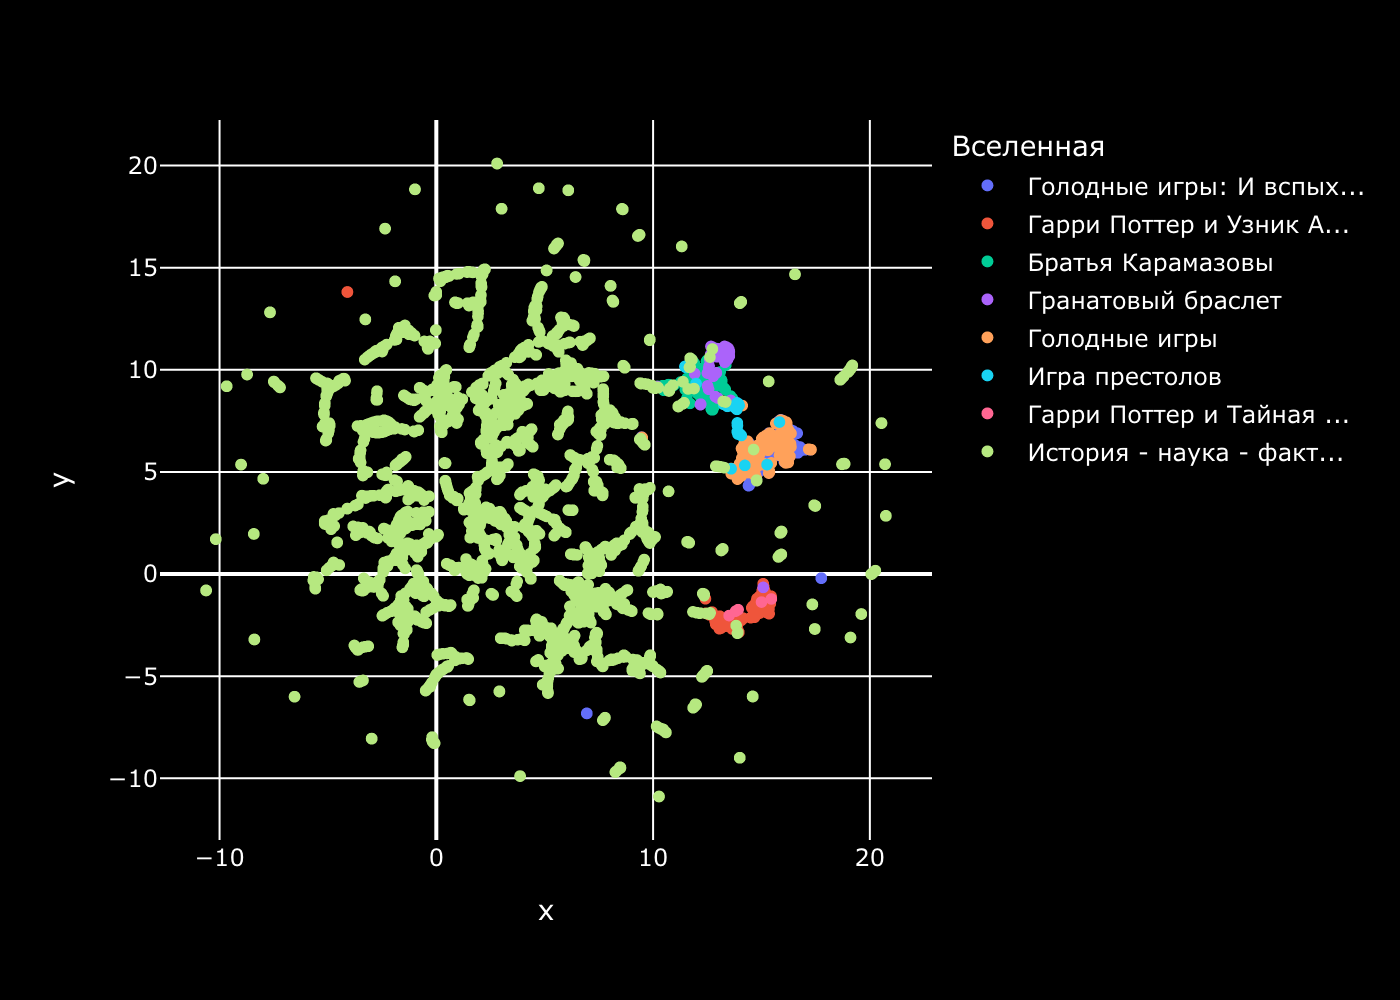
\includegraphics[width=\columnwidth]{figures/clustering-e5-base.png} % Используем ширину одной колонки
    \caption{Кластеризация полного набор данных $D$, включающего в себя как $D_u$,  так и $D_v$}
    \label{fig:clustering-e5-base}
\end{figure}

Ниже представлена таблица \eqref{tab:tokensdist} со статистикой по распределению длин параграфов, запросов, ключевых слов и их пересечения.

\paragraph{Обозначения}
Для каждого параграфа $d_j$ имеется соответствие: $I_j$ - список индексов вопросов $q_i$, ответ на которые содержится в $d_j$. 
Кроме того, каждому параграфу $d_j$ сопоставлены ключевые слова и объяснения $K_j$.

Формально, для каждого параграфа $d_j$ имеется (возможно пустое) множество ключевых слов и их контекстных объяснений, которые обозначются как 
$k_s$ и $e_s$.

\begin{align}
K_j = \{(k^j_{s1}, e^j_{s1}), (k^j_{s2}, e^j_{s2}), \cdots\}
\end{align}

Отметим,что каждое ключевое слово $k_s$ является строгой подстрокой параграфа $k_s \subset d_j$, а объяснение $e_s$, в общем случае, не обязано - $e_s \not\subset d_j$
\paragraph{Статистика}
% \begin{align}
%     L_{Q} &= \frac{1}{|Q|}\sum_{i=1}^{|Q|} |q_i| \\
%     L_{D} &=\frac{1}{|D|}\sum_{j=1}^{|D|} |d_j| \\
%     L_{QD} &= \sum_{j=1} \sum_{i\in I_j} \frac{|q_i \cap d_j|}{|d_j|} \\
%     L_{KD} &= \sum_{j=1} \sum_{s\in K_j} \frac{|k_s \cap d_j|}{|d_j|} \\
%     L_{KED} &= \sum_{j=1} \sum_{s\in K_j} \frac{|k_s \cup e_s \cap d_j|}{|d_j|}
%     \label{eq:coverage}
% \end{align}
\begin{equation}\label{eq:coverage}
    \begin{aligned}
        L_{Q} &= \frac{1}{|Q|}\sum_{i=1}^{|Q|} |q_i|, \\
        L_{D} &= \frac{1}{|D|}\sum_{j=1}^{|D|} |d_j|, \\
        L_{QD} &= \sum_{j=1} \sum_{i \in I_j} \frac{|q_i \cap d_j|}{|d_j|}, \\
        L_{KD} &= \sum_{j=1} \sum_{s \in K_j} \frac{|k_s \cap d_j|}{|d_j|}, \\
        L_{KED} &= \sum_{j=1} \sum_{s \in K_j} \frac{|k_s \cup e_s \cap d_j|}{|d_j|}.
    \end{aligned}
\end{equation}
В уравнениях \eqref{eq:coverage} определяются статистики, важные для подсчета и обоснования важности учета алгоритма (мотивы их ввода более подробно объяснены далее). 
$L_{Q}, L_{D}$ - это длины (среднее) запросов и параграфов соответственно. $L_{QD}$ - среднее покрытие (пересечение) слов из запросов с релевантными параграфами.
$L_{KD}, L_{KED}$ - это процент покрытия токенов параграфа его соответствующими ключевым словами (без объяснениний) и ключевыми словами вместе с объяснениями.
\begin{table}[h]
    \centering
    \begin{tabular}{l|ccccc}
        \textbf{} & \textbf{$L_{Q}$} & \textbf{$L_{D}$} & \textbf{$L_{QD}$} & \textbf{$L_{KD}$} & \textbf{$L_{KED}$} \\
        \hline
        \textbf{$D_{u}$}  &$22.48$ &$144.125$  &$4.77\%$  &$8.64\%$  & $21.45\%$ \\
        \textbf{$D_{v}$}  &$24.99$  &$100.73$  &$6.03\%$  &$8.96\%$  & $23.69\%$ \\
        \textbf{$D_{uv}$} &$23.66$  &$123.73$  &$5.3\%$  &$8.79\%$  & $22.5\%$ \\
    \end{tabular}
    \caption{Распределение ключевых статистических метрик относительно $D_u$ и $D_v$ наборов данных}
    \label{tab:tokensdist}
\end{table}

Несмотря, на очевидную разницу двух наборов данных -  $L_D(D_u)=144.125$ и $L_D(D_v)=100.73$, их стилистику, речевые обороты и другие лингвистические характеристики, отдельно взятый набор $D_u$ сам по себе уникален с точки зрения поиска. 
Так, например, ниже представлена кластеризация подмножества $\hat{D_u} \subset D_u$ произведений $D_u$ в количестве $|\hat{D_u}|=1530$ примеров.

\begin{figure}[ht]
    \centering
    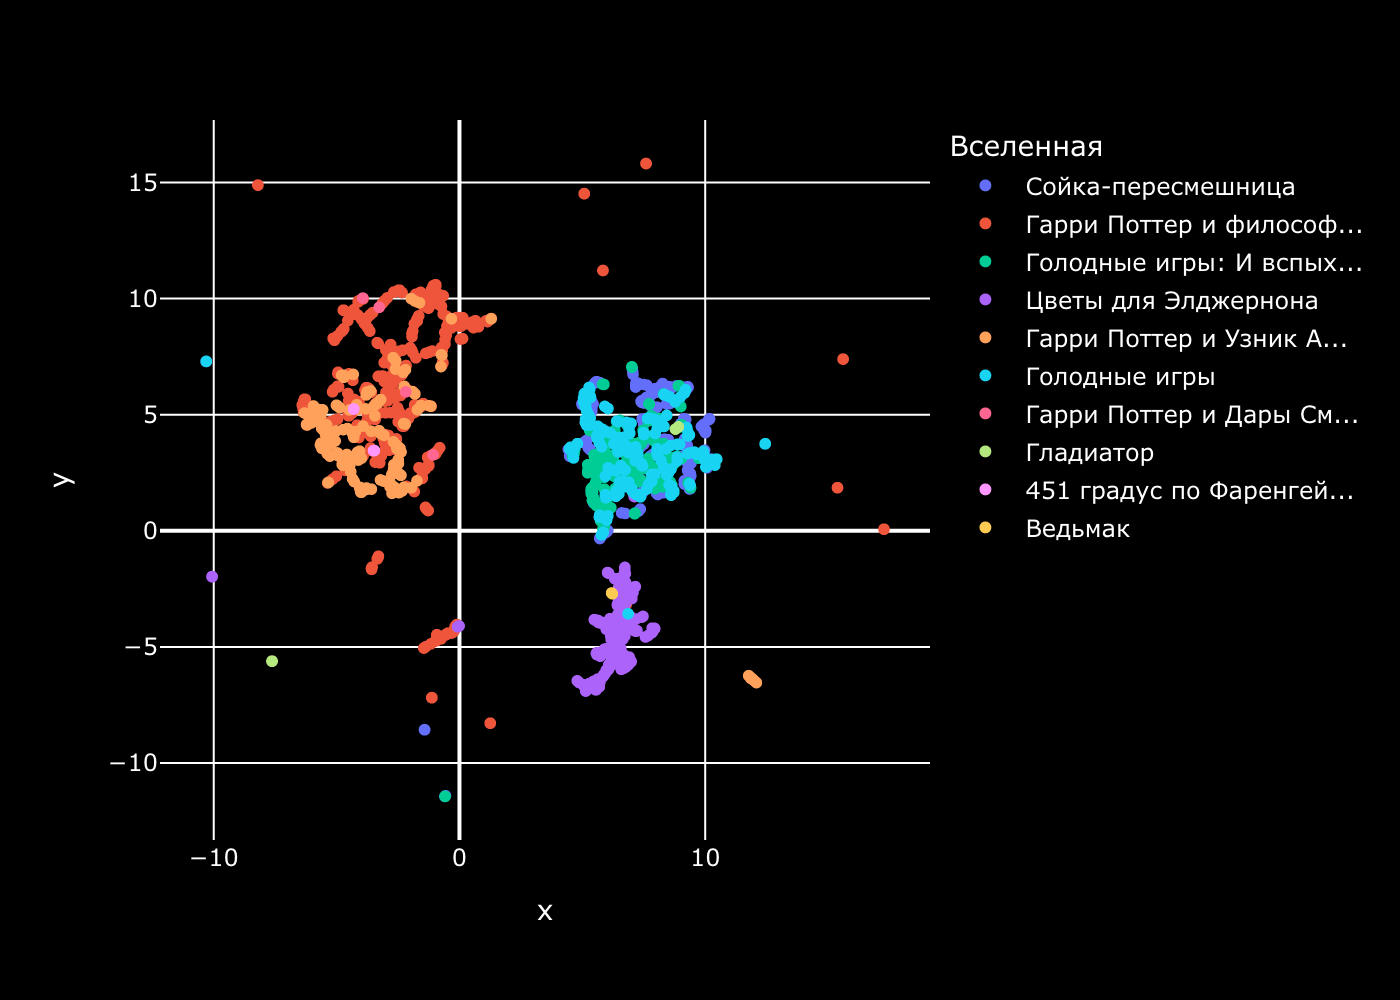
\includegraphics[width=\columnwidth]{figures/clustering_model=[e5]_dataset=[universe].png} % Используем ширину одной колонки
    \caption{Демонстрация кластеризации набора данных $D_u$}
    \label{fig:clustering-e5-base-universe}
\end{figure}

\section{Алгоритм (Retriever)}
\label{sec:retriever}

В данной статье основной фокус представлен на то, как можно улучшить уже существующий (пред-обученный) компонент поиска $R$ \eqref{eq:retriever}.
Получив на вход коллекцию из $|D|=N$ документов (параграфов), задача поиска $R$ проиндексировать эти данные в непрерывное метрическое пространство, например, Евклидово - $\Re^n$, 
таким образом, чтобы при входящем запросе $q_i$ выдавать $top_k$ ближайших $top_k\leq 20$ параграфов, подходящих по смыслу.


\subsection{Метрическое пространство}
При работе поисковой системы, на вопрос $q_i$ сопоставляется нейронной моделью $n$-мерный вектор $\vec{v}_i$.
Далее происходит поиск ближайшего векторов, используя алгоритм ближайшего соседа \textit{HNSW} \cite{enwiki:hsnw}. Несмотря на большое разнообразие метрик, в данной работе используется простое скалярное произведение.

\begin{align}
    S(\vec{h_i}, \vec{h_j})=F_{\omega}(q_i) \cdot F_{\omega}(d_j)
    \label{eq:cosine-measure}
\end{align}
% uses a dense encoder $E_P(\cdot)$ which maps any text passage to a $d$-dimensional real-valued vectors and builds an index for all the $M$ passages that we will use for retrieval.
% At run-time, \model/ applies a different encoder $E_Q(\cdot)$ that maps the input question to a $d$-dimensional vector, and retrieves $k$ passages
% of which vectors are the closest to the question vector. We define the similarity between the question and the passage using the dot product of their vectors:
% \begin{align}
%     \mathrm{sim}(q, p) = E_Q(q)^{\intercal} E_P(p).
%     \label{eq:sim}
% \end{align}
% Although more expressive model forms for measuring the similarity between a question and a passage do exist, such as networks consisting of multiple layers of cross attentions, the similarity function needs to be decomposable so that the representations of the collection of passages can be pre-computed.
% Most decomposable similarity functions are some transformations of Euclidean distance (L2). For instance, cosine is equivalent to inner product for unit vectors and the Mahalanobis distance is equivalent to L2 distance in a transformed space.
% Inner product search has been widely used and studied, as well as its connection to cosine similarity and L2 distance~\cite{mussmann2016learning,ram2012maximum}.
% As our ablation study finds other similarity functions perform comparably (Section~\ref{sec:sim_loss}; Appendix~\ref{sec:alt-sim}), we thus choose the simpler inner product function and improve the dense passage retriever by learning better encoders.

\paragraph{Векторные модели отображения (Encoders)}
Реализация нейронного поиска может быть реализована любой нейросетью, но в данной статье выбрано семейство моделей 
\textit{E5} \cite{e5} по двум причинам. Во-первых - они мультиязычны, что необходимо для набора данных $D_u$, т.к. он содержит как англоязычные, так и русскоязычные параграфы (и вопросы к ним соответственно).
Во-вторых, семейство моделей \textit{E5} является SOTA на задаче поиска ``\textit{Semantic Textual Similarity}'' согласно бенчмаркам ``\textit{MTEB}'' \cite{mteb} и ``\textit{RuMTEB}'' \cite{rumteb}.
В третьих, модели \textit{E5} были дополнительно пред-обучены ассиметрично, путем добавления двух разных префиксов к запросам и параграфам. А именно, для запроса использовался используется
$p_{q}=\text{query:}$, а для параграфа, который добавляется в индекс - $p_{d}=\text{passage:}$.

Таким образом, как для параграфов $d_j$, так и для запросов $q_i$, используется ассиметричная модель поиска \textit{E5} (``Small'', ``Base'', ``Large'') с модификацией префикса, согласно предобучению самой модели \cite{e5}.
\begin{align}
    \vec{h}_j&=F(d_j) = F_{\omega}(p_d + d_j) \\
    \vec{h}_i&=F(q_i) = F_{\omega}(p_q + q_i)
    \label{eq:e5}
\end{align}

\paragraph{Поиск ближайшего соседа (ANN)}
Во время работы всей системы, используется сопоставление векторной моделью поиска $F_{\omega}$ \eqref{eq:e5} запроса $q_i$ и, по полученному вектору $\vec{h}_i$ производится 
поиск по индексу, в который были вложены вектора параграфов этой же самой моделью \eqref{eq:e5}. Для реализации поиска алгоритма ближайшего соседа (ANN) применяется реализация 
\textit{Weaviate} \cite{weaviate} - эффективная реализация поиска через \textit{HNSW} алгоритм \url{enwiki:hsnw}, позволяющий индексировать 
данные миллиардных порядков $|D|\ge 10^8$. Фактически, получая на вход запрос $q_i$, через нейронную модель производится вектор $\vec{h}_i$ и, 
среди всех векторов индекса ищется $top_k$ ближайших \eqref{eq:cosine-measure} в метрическом (скалярном) пространстве $\Re^n$, наиболее близких к $\vec{h}_i$.

\subsection{Алгоритм (pipeline)}\label{sec:algo}
На этапе индексации, получив на вход параграфы $D=\{d_j\}$ происходит извлечение ключевых слов и их объяснений в контексте параграфа $d_j$ \eqref{eq:keywords}.

\begin{align}
    \mathrm{Keywords}(d_j) = \{\{k^j_1, e^j_1\}, \cdots, \{k^j_{\sigma(j)}, e^j_{\sigma(j)}\}\}
    \label{eq:keywords}
\end{align}

Извлечение ключевых слов может быть реализовано разными способами, в данной работе использовалась модель \textbf{GPT4-turbo}, с промптом указанным в \href{https://github.com/atomicai/justatom/blob/86f405cf9c6b5bd5cf484636e4d4dcbd10ec0ca1/justatom/running/prompt.py#L16}{prompts.py}. Далее, 
происходит стандартный процесс сопоставления векторов $\vec{v}_j = F_{\omega}(d_j)$ \eqref{eq:e5} указанной моделью и добавление в ANN индекс, используя \textit{Weaviate} \cite{weaviate}.
Самое интересное происходит во время поиска. Для реализации поиска $top_k$ ближайших параграфов к заданному вопросу $q_i$ сначала, как обычно, 
сопоставляется вектор для запроса $\vec{v}_q=F_{\omega}(q_i)$ и, впоследствии делается поиск $top_p >> top_k$ ближайших соседей. Это позволяет учесть большую часть 
всех семантически близких параграфов и, \underline{уже среди ближайших} $top_p$ выбрать необходимые $top_k$, ранжируя их в соответствии с необходимой полнотой выдачи ключевых слов. Отдельный интерес 
представляет функция ранжирования - $\phi$. 

\begin{align}
    \phi& = \gamma_1 \times \phi_s + \gamma_2 \times \phi_r, \gamma_i \in (0, 1)
    \label{eq:phi-global}
\end{align}

В \eqref{eq:phi-global} представлены две функции $\phi_s$ и $\phi_r$. Первая из них - $\phi_s$ это, фактически семантический результат близости векторов. Вторая - 
$\phi_r$ реализует вклад ``ключевых слов''. Вклад ключевых слов можно реализовать множеством способов, однако среди всех перебранных, наилучшей оказалась следующая реализация $\phi_s$:

\begin{small}
\begin{align}
    \sum_{k^j_s, e^j_s \in K_j \cap q_i} \frac{1.0}{\ln(1 + p_{\xi}(w_i))} \times [\sum_{k^j_s, e^j_s \in K_j} \frac{1.0}{\ln(1 + p_{\xi}(w_i))}]^{-1}
\end{align}
\label{eq:idfrecall}
\end{small}

Ранжирование \eqref{eq:idfrecall} представляет собой численный ответ на вопрос: \textbf{Какую часть важных слов контекста ``покрыл'' запрос?}. Так, рассмотрим пример:
При полном совпадении ключевых слов параграфа $K_j$ и запроса $q_i$ - числитель совпадает со знаменателем и $\phi_s(q_i, K_j)=1.0$. Если же, наоборот, 
общих слов нет вообще, то $\phi_r(q_i, K_j)=0.0$. Рассмотрим следующий пример с $q_i$ и выданным контекстом $d_j$, как показано в 
\ref{fig:sample-hunger-games}. $p_{\xi}(w_i)$ - это частота встречаемости слова в контексте. В 
примере из \ref{fig:sample-hunger-games} $p_{\xi}(w_4)=2$ т.к. слово ``арена'' встречается дважды. Оно также входит в запрос $q_i$, поэтому в итоговой сумме будет учтено и в числителе.
Слова: ``трибуты'' и ``мятеж'' не входят в запрос $q_i$, поэтому их учет будет лишь в знаменателе \eqref{eq:idfrecall}. Посчитаем для этого примера полное значение ранжирования $\phi_r$.
\begin{small}
    \begin{align}
        \Omega_1=\frac{1}{\ln(1 + p_{\xi}(w_1))}\approx 1.4427 \\
        \Omega_2=\frac{1}{\ln(1 + p_{\xi}(w_2))}\approx 1.4427 \\
        \Omega_3=\frac{1}{\ln(1 + p_{\xi}(w_3))}\approx 0.9102\\
        \Omega_4=\frac{1}{\ln(1 + p_{\xi}(w_4))}\approx 0.9102
    \end{align}
    \label{eq:calculation-for-sample}
\end{small}

Таким образом, финальная метрика равна:

\begin{small}
    \begin{align}
        \phi_s(q_i, d_j)=\frac{\Omega_1 + \Omega_4}{\Omega_1+\Omega_2+\Omega_3+\Omega_4}\approx 0.5
    \end{align}
\end{small}

Если же из запроса убрать слово ``арена'', что сделает запрос более расплывчатым, т.к. теперь смысл может быть немного другим, то ранжирование будет меньше и равно примерно $\approx 0.3065$

\begin{figure}[ht]
    \centering
    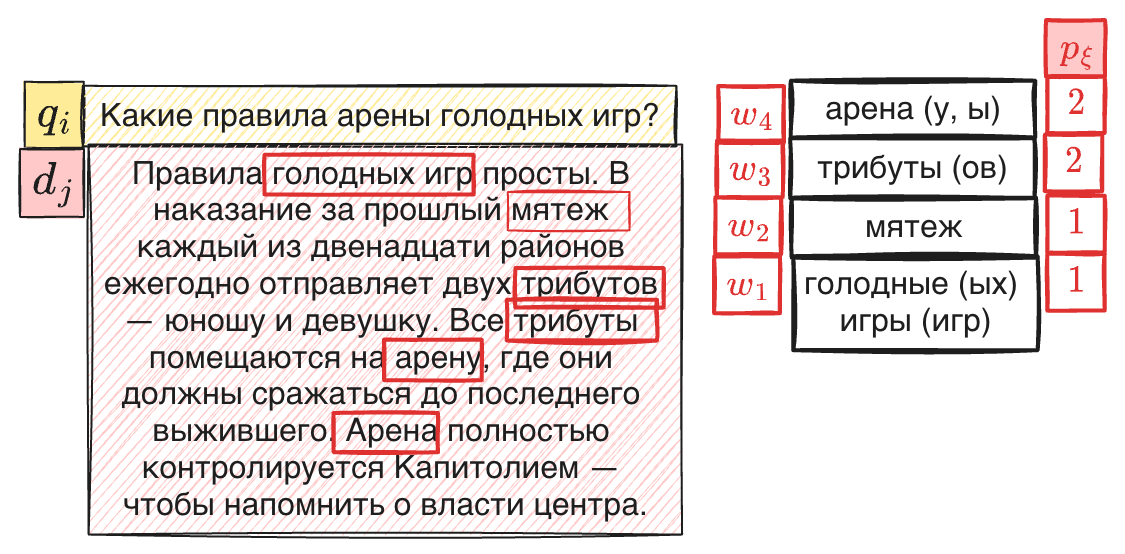
\includegraphics[width=\columnwidth]{figures/sample-hunger-games.png} % Используем ширину одной колонки
    \caption{Демонстрация функции $\phi_s$ на запросе к вселенной  \href{https://w.wiki/DQ\$z}{``Голодные игры''}}
    \label{fig:sample-hunger-games}
\end{figure}


\subsection{Подбор гипер-параметра ($\gamma$)}\label{sec:algo}

Отдельным пунктом рассмотрим, как эффективно подобрать $\gamma$ в \eqref{eq:phi-global}. 
Из-за фиксированного векторного отображения \eqref{eq:e5} фактически уравнение \eqref{eq:phi-global} является функционалом с 
двумя переменными $\gamma_1, \gamma_2$:

\begin{align}
    f(\gamma_1, \gamma_2)& = \gamma_1 \times \phi_s + \gamma_2 \times \phi_r
    \label{eq:gamma-func-forward}
\end{align}

Требуется максимизировать для ``правильных'' пар, т.е. таких $\{q_i, d^+_i\}_{i=1}^{N}$ - требуется оптимально подобрать $\gamma$, 
чтобы максимизировать $f(\gamma_1, \gamma_2) \rightarrow max$. Перегруппировав неизвестные $\gamma_1, \gamma_2$ в \eqref{eq:gamma-func-forward} и сгруппировав его для каждой пары 
$\{q_i, d_i^{+}\}_{i=1}^{N}$, получаем систему пере-определенных линейных уравнений. Такая система, очевидно, не решается алгебраически, а любое ее приближение 
будет крайне ошибочным. В связи с этим, для решения мы используем метод градиентного спуска, до-обучая систему в соответствии с той же функцией ошибки, 
которая использовалась при обучении пред-обученных моделей \textit{E5} \cite{e5}. Таким, образом, для отдельно взятого под-множества (батча) 
$S_i = \{\{q_i, d_i\}, \{q_{i+1}, d_{i+1}\}, \cdots, \{q_{i+|bs| - 1}, d_{i+|bs| - 1}\}\}$, требутеся максимизировать итоговое ранжирование или, что тоже самое, 
минимизировать среднее отклонение по всем батчам $S_i$, для всех $\forall i \in \{1, \cdots, N\}$.
\begin{small}
\begin{align}
   L_{\gamma_1, \gamma_2} = \sum_i-\frac{1}{|S_i|} \sum \log \frac{e^{\phi(q_i, d_i)}}{e^{\phi(q_i, d_i^{+})} + \sum_{j\neq i}e^{\phi(q_i, d_j)}}
    \label{eq:gamma-func}
\end{align}
\end{small}

Как это часто бывает, в некоторых взвешенных функциях, которые суммируют вклад нескольких, отдельно взятых функций, часто 
применяют более простые ранжирования. Так, например, в нашем случая, может показаться, что вполне хватит и одной переменной - $\gamma_1$, вместо двух - 
$\gamma_1, \gamma_2$, выраженная следующим образом: $\gamma_2=1 - \gamma_1$. Однако, как показано ниже на графике, дополнительная связь, не 
помогает максимизировать \eqref{eq:gamma-func-forward}, оставляя большой разрыв между графиками сравнения.

\begin{figure}[ht]
    \centering
    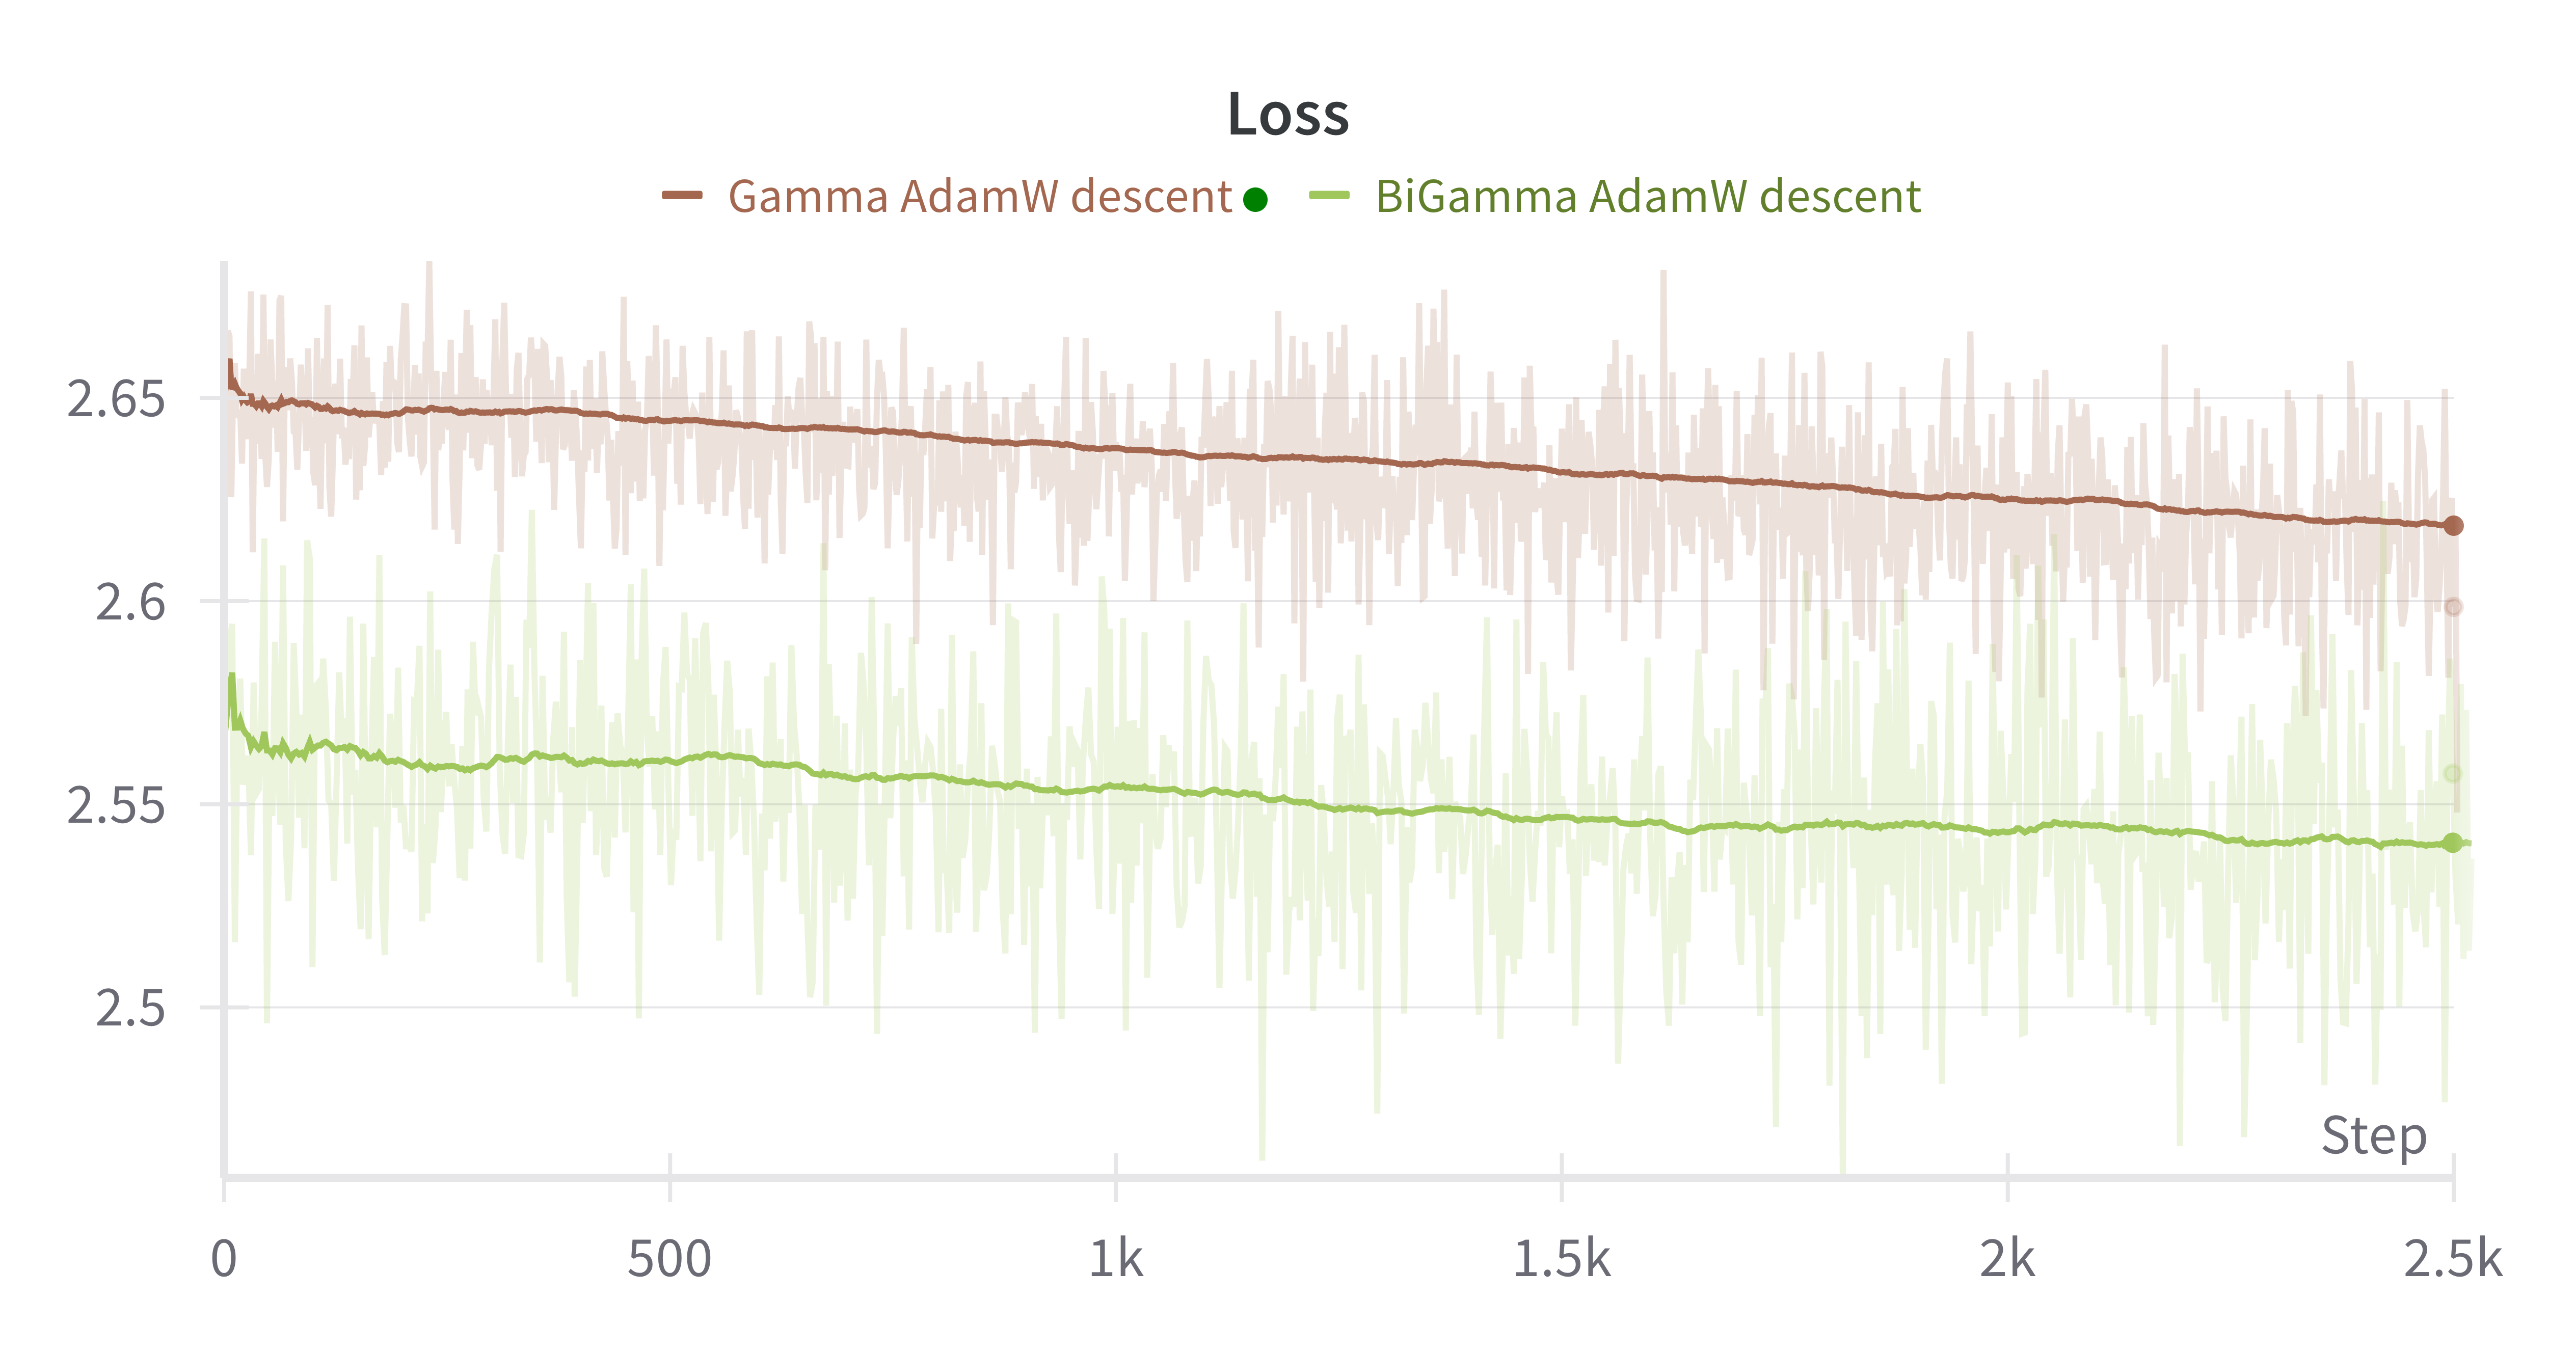
\includegraphics[width=\columnwidth]{figures/Loss-BiGamma-vs-Gamma.png} % Используем ширину одной колонки
    \caption{Сравнение характера функции потерь в \eqref{eq:gamma-func} в разные случаях: $\gamma_1, \gamma_2$ и $\gamma_1 + \gamma_2=1$}
    \label{fig:comparison-gammas}
\end{figure}

\subsection{Сравнительный анализ метрик}

Для функции ранжирования, вполне мог бы подойти и сам текст параграфа. Действительно, код и оставшаяся часть алгоритма никак бы не изменились. 
Однако выбор самого текста параграфа влечет за собой некоторые изъяны, и как показано на графике ниже, аномальные всплески сильно ``ухудшают'' общую метрику, 
приоритезируя выдачу по ключевым словам. Так, например, для набора данных $D_u$ показано сравнения $\phi_r$ на контексте документа и его ключевых словах:

\begin{figure}[ht]
    \centering
    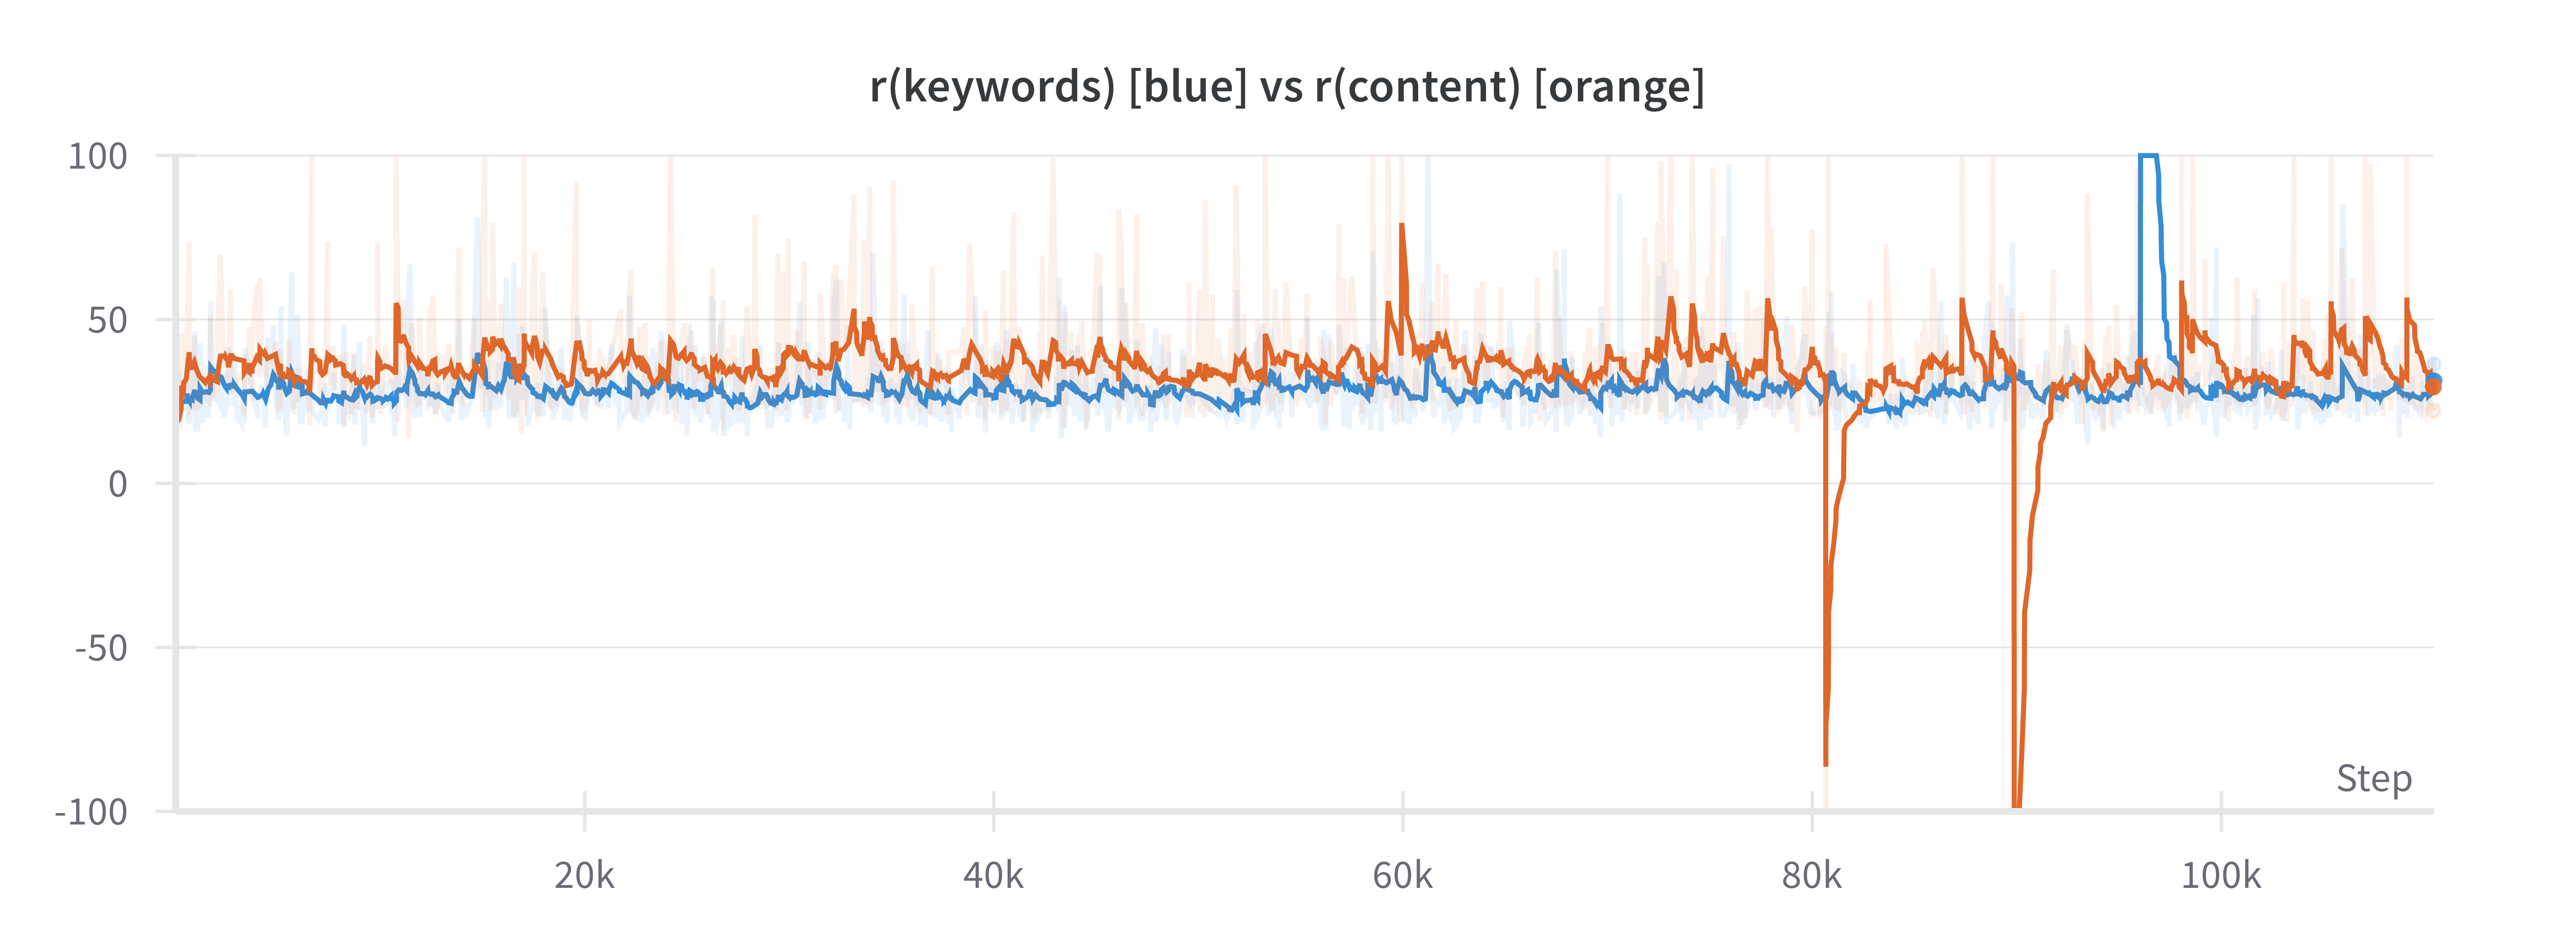
\includegraphics[width=\columnwidth]{figures/idf-recall-content-vs-keywords.png} % Используем ширину одной колонки
    \caption{Сравнение ранжирующей функции $\phi_r$ на примере данных $D_u$}
    \label{fig:comparison-phir-content-vs-keywords}
\end{figure}

Подытоживая вышесказанное, весь алгоритм, в таком случае, визуально представлен ниже:

\begin{figure}[ht]
    \centering
    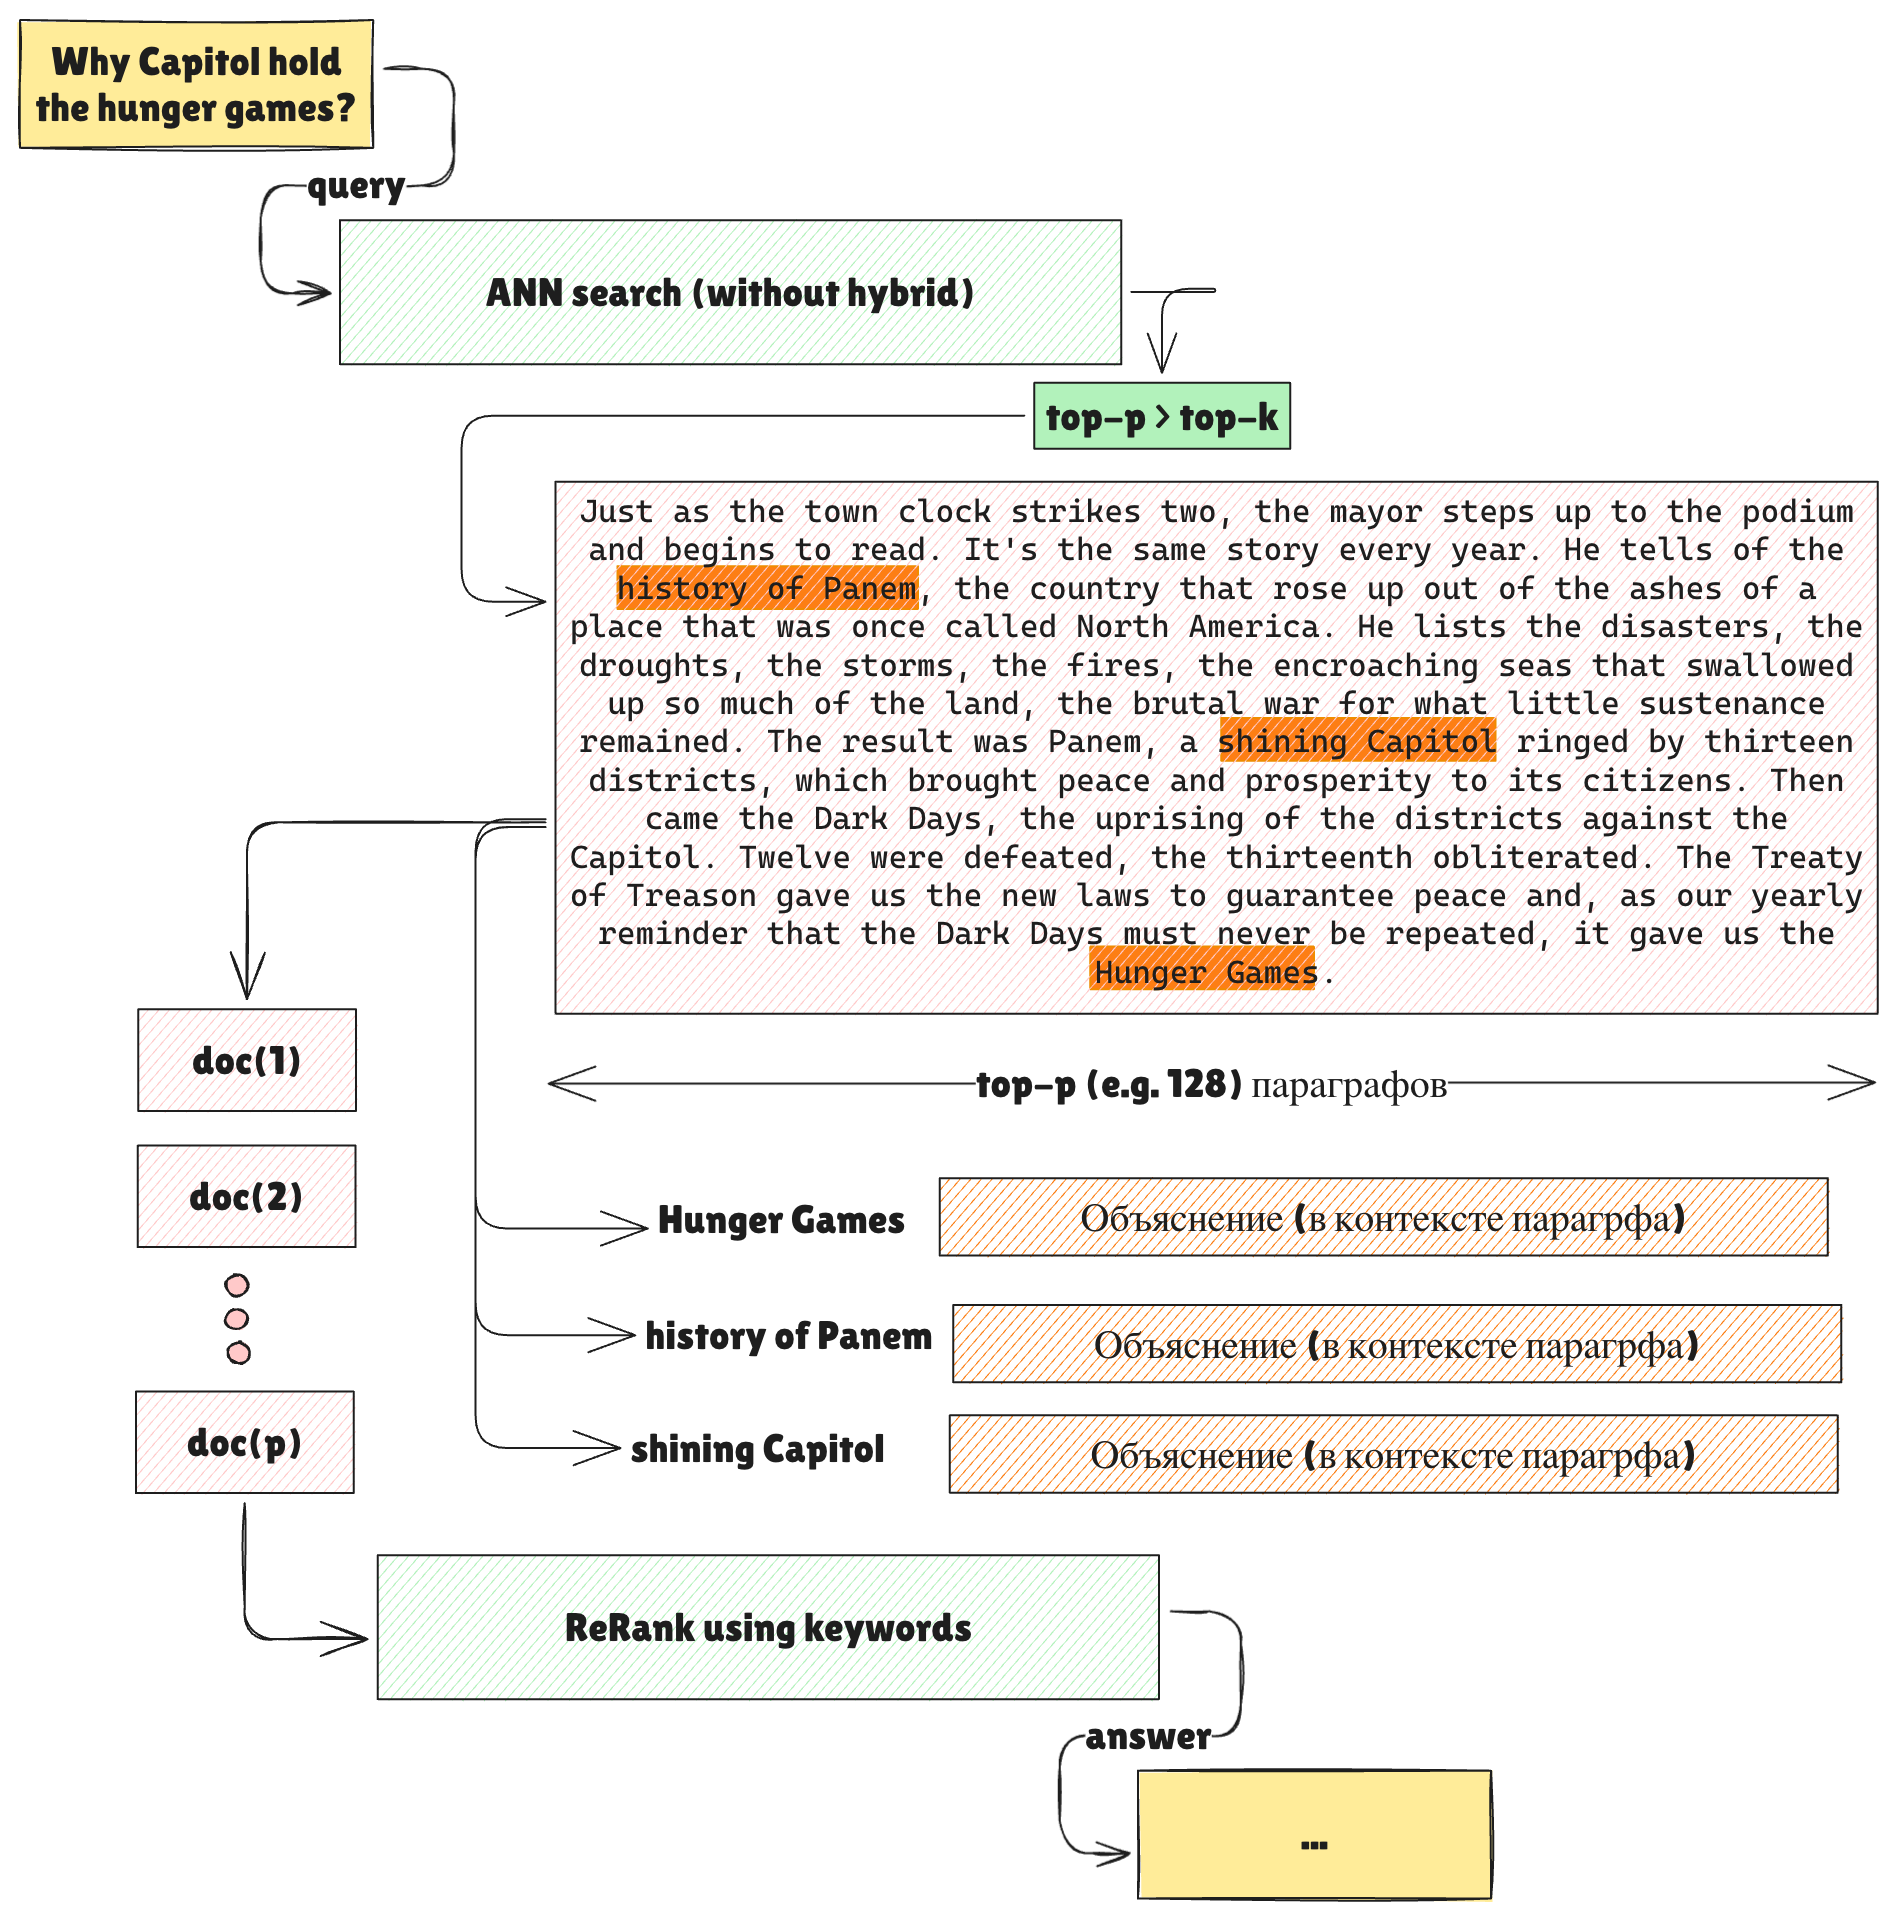
\includegraphics[width=\columnwidth]{figures/top-k-top-p.png} % Используем ширину одной колонки
    \caption{Визуальная демонстрация выбора $top_k \leq top_p$ среди $top_p$ ближайших параграфов}
    \label{fig:comparison-phir-content-vs-keywords}
\end{figure}

Полный псевдо-код описан в \ref{alg:pipeline_for_atomic}.

\begin{figure*}[ht]
% \centering
\makebox[\textwidth]{ % Обеспечивает использование всей ширины страницы
\begin{minipage}{\textwidth}
\begin{algorithm}[H] % Убедитесь, что \caption находится здесь
    \caption{Pipeline for ATOMIC}
    \label{alg:pipeline_for_atomic}
    \begin{algorithmic}[1] % Нумерация строк
    \Procedure{Retrieve}{$Q=\{q_1, q_2, \cdots \}, top_K, top_P$}
        % \State \textbf{$\gamma_1, \gamma_2$} computed $\gets$  \eqref{eq:gamma-func}
        \State \textbf{Compute } $\gamma_1, \gamma_2$ \textbf{ using } \eqref{eq:gamma-func}
        \ForAll{$q_i$ in $Q$}
                    \State \textbf{Maps} $\vec{q_i} \gets F_{\omega}(q_i)$
                    \State \textbf{Search} $D_i \gets R_e({\vec{q_i}})$ 
                    \Comment{Perform ANN search finding $top_P$ closest paragraphs}\\
                    \Comment{Assign them to the variable $D_i = \{d^i_1, \dots, d^i_{top_p}\}$}


                    \ForAll{$d^i_j$ in $D_i$}
                            \State $s^i_j \gets f_{\gamma_1, \gamma_2}(q_i, d^i_j)$
                    \EndFor
                    
                    % --- НОВЫЙ БЛОК: сортируем и берем Top-k ---
                    \State \textbf{Sort} $\hat{D_i} \gets \{d^i_1, \dots, d^i_{top_k}\}$ 
                    \Comment{Let's sort $top_P$ paragraphs returned from $D_i$ according to $s^i_j$}\\
                    \Comment{Select $top_K \leq top_P$ sorted paragraphs from $D_i$}

                    \State \textbf{Yield} $\hat{D_i}$
                    \Comment{Return (yield) the given $top_k$ paragraphs for the $q_i$}
        \EndFor
    \EndProcedure
    \end{algorithmic}
\end{algorithm}
\end{minipage}
}
\end{figure*}


\section{Метрики}
\label{sec:metrics}

Данный раздел посвящен выявлению особенностей и численному сравнению алгоритмов. В последующих разделах везде подразумеваются следующие обозначения:

\begin{itemize}
    \item $R_k$ - поиск, реализующий алгоритм \textit{BM25} \cite{robertson2009probabilistic}
    \item $R_e$ - поиск ближайшего соседа (ANN), использующий реализацию \textit{Weavaite} \cite{weaviate} алгоритмом \textit{HNSW} \url{enwiki:hsnw}
    \item $R_h$ - гибридный поиск, совмещающий первых два подхода, с наилучшим выбранным порогом $\theta$.
    \item $R_{\gamma}$ - поиск ближайшего соседа (ANN), используюший ранжирование $f(\gamma_1, \gamma_2)$ \eqref{eq:gamma-func}
\end{itemize}


\subsection{Выбор ключевых слов}
\label{sec:keywords-vs-content}

Для функции ранжирования, вполне мог бы подойти и сам текст параграфа. Действительно, код и оставшаяся часть алгоритма никак бы не изменились. 
Однако выбор самого текста параграфа влечет за собой некоторые изъяны, и как показано на графике ниже, аномальные всплески сильно ``ухудшают'' общую метрику, 
приоритезируя выдачу по ключевым словам. Так, например, для набора данных $D_u$ показано сравнения $\phi_r$ на контексте документа и его ключевых словах:

% \begin{figure}[ht]
%     \centering
%     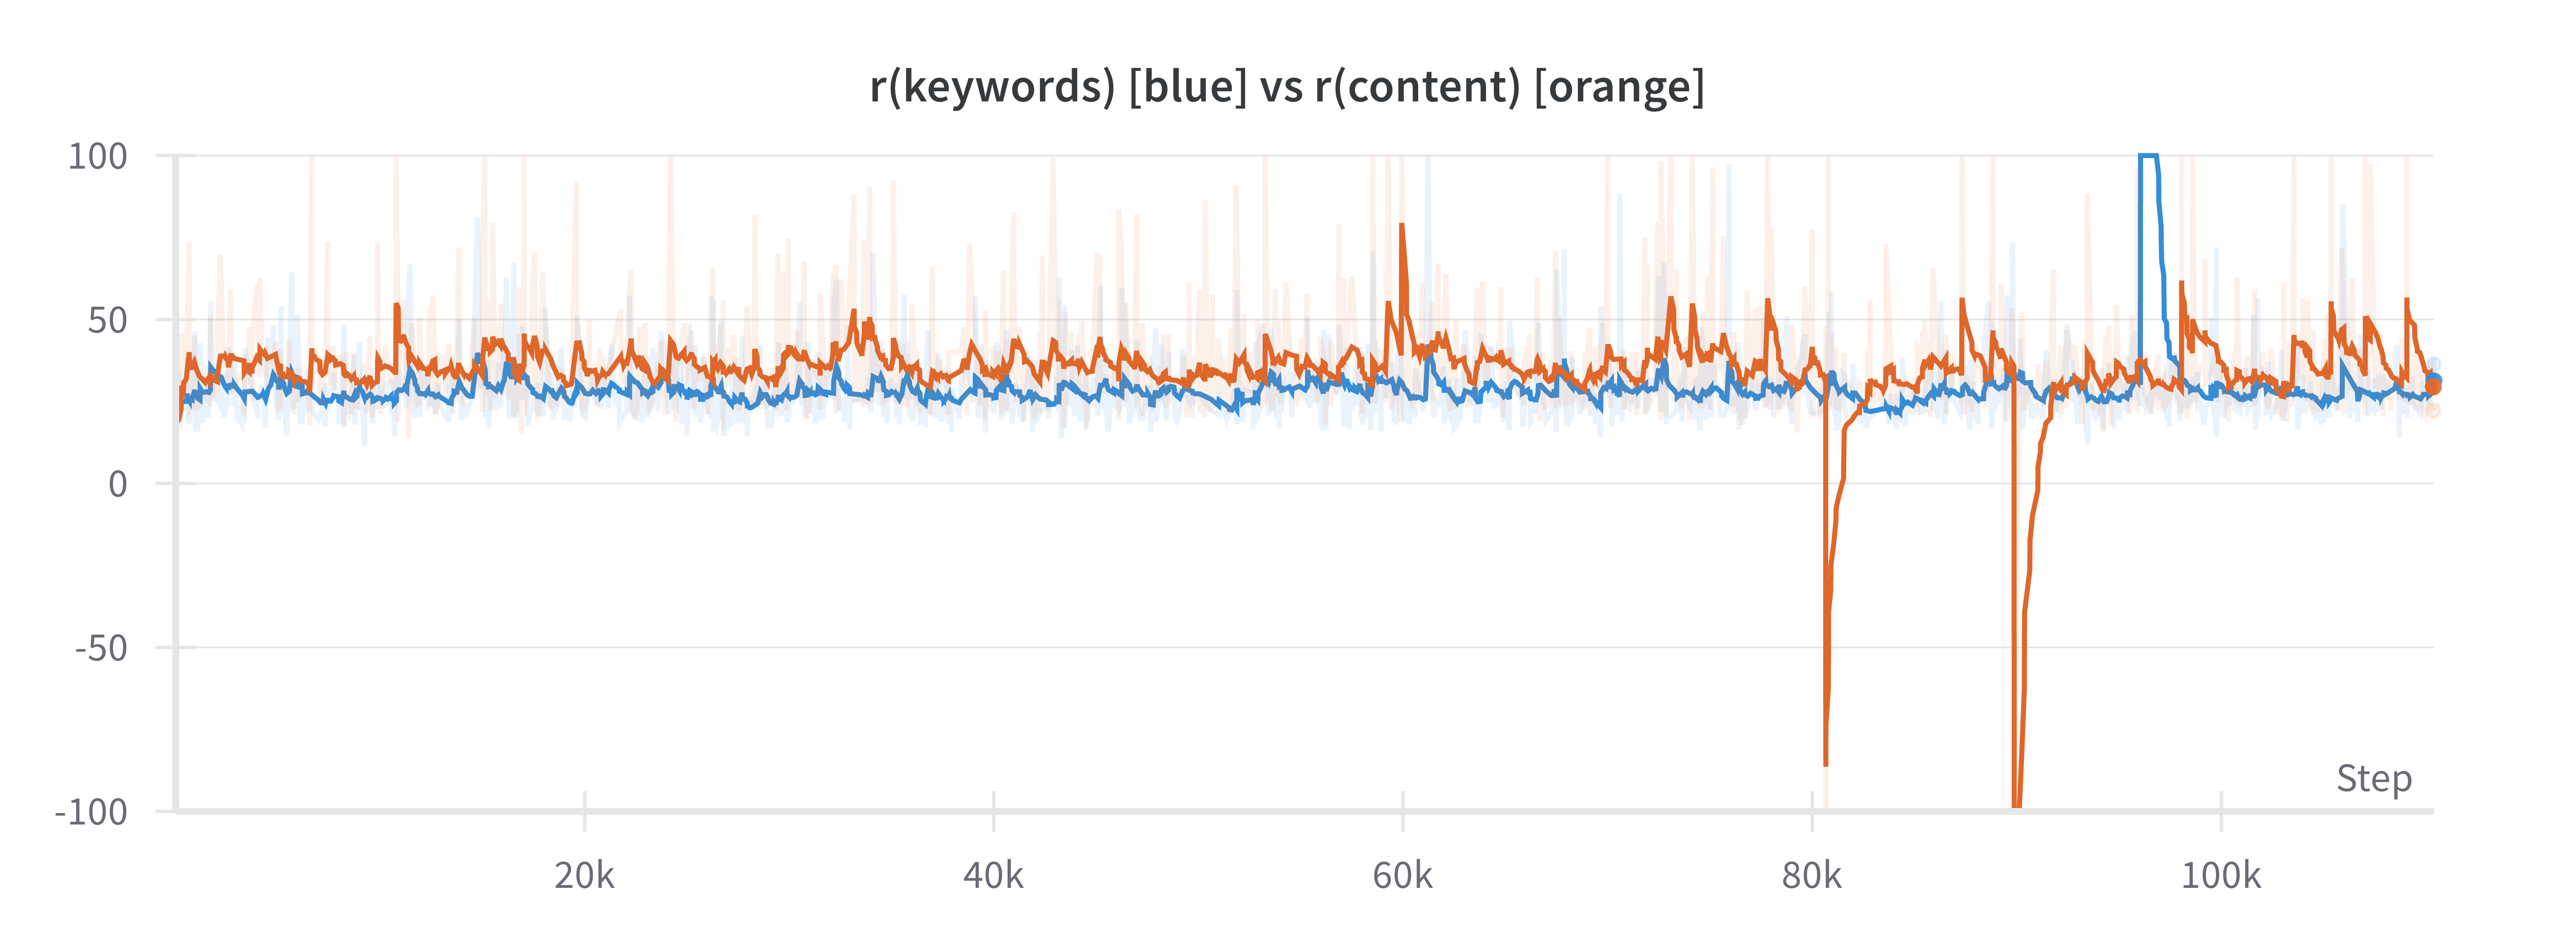
\includegraphics[width=\columnwidth]{figures/idf-recall-content-vs-keywords.png} % Используем ширину одной колонки
%     \caption{Comparison of $\phi_r$ using $D_u$ dataset}
%     \label{fig:comparison-phir-content-vs-keywords}
% \end{figure}


\subsection{Результаты}
\label{sec:final-metrics}

Ниже, приведены основные результаты сравнения, подтверждающие гипотезу о том, что гибридный поиск $R_h$(с наилучшим коэффициентом $\theta$) 
показывает результаты хуже, чем предложенный в статье алгоритм - $R_{\gamma}$, основанный на дополнительном ранжировании, выбирающий $top_p$ и дополнительно 
ранжирующий результаты через $\gamma_1, \gamma_2$.

В таблицах ~\ref{tab:hitrate-small} ~\ref{tab:hitrate-base} ~\ref{tab:hitrate-large} представлены результаты сравнения на выборке данных из $D_u$, $D_v$ для моделей семейства \textit{E5} \cite{e5} размеров \textit{$E5_{small}$}, \textit{$E5_{ base}$} и \textit{$E5_{large}$} соответственно.
\begin{table}[ht]
    \centering
    \begin{tabular}{lcccccc}
        \hline
        & \textbf{HitRate@k (\(D_u\))} & \textbf{HitRate@k (\(D_v\))} \\
       \hline
       \(R_k\)      &  0.49&  0.79 \\
       \(R_e\)      &  0.53&  0.89\\
       \(R_h\)      &  0.56&  0.91\\
       \(R_{\gamma}\) &  \textbf{0.60}&  \textbf{0.93}\\
       \hline
       \end{tabular}
    \caption{Метрика $HitRate@k$ на примере модели $E5_{small}$ \cite{e5}}
    \label{tab:hitrate-small}
\end{table}
\begin{table}[ht]
    \centering
    \begin{tabular}{lcccccc}
        \hline
        & \textbf{HitRate@k (\(D_u\))} & \textbf{HitRate@k (\(D_v\))} \\
       \hline
       \(R_k\)      &  0.49&  0.79 \\
       \(R_e\)      &  0.58&  0.90\\
       \(R_h\)      &  0.61&  0.92\\
       \(R_{\gamma}\) &  \textbf{0.633}&  \textbf{0.93}\\
       \hline
       \end{tabular}
    \caption{Метрика $HitRate@k$ на примере модели $E5_{base}$ \cite{e5}}
    \label{tab:hitrate-base}
\end{table}
\begin{table}[ht]
    \centering
    \begin{tabular}{lcccccc}
        \hline
        & \textbf{HitRate@k (\(D_u\))} & \textbf{HitRate@k (\(D_v\))} \\
       \hline
       \(R_k\)      &  0.49&  0.79 \\
       \(R_e\)      &  0.64&  0.92\\
       \(R_h\)      &  0.66&  0.93\\
       \(R_{\gamma}\) &  \textbf{0.681}&  \textbf{0.94}\\
       \hline
       \end{tabular}
    \caption{Метрика $HitRate@k$ на примере модели $E5_{large}$ \cite{e5}}
    \label{tab:hitrate-large}
\end{table}

\noindent
\textbf{Universe Question ($D_u$)}~\cite{repojustatom} - вопросы и параграфы, основанные на вселенных из книг, игр, фильмов или сериалов.
Набор данных был составлен экспертами, которые были погружены в эти вселенные. Помимо уникальной лингвистической структуры, речевыми оборотами, 
этот датасет предсталяет особую трудность для адаптации из-за сложности в токенизации имен собственных, заклинаний и лексическим сдвигом от формального повествования. 
Так, например, в таких произведениях как 
\href{https://en.wikipedia.org/wiki/Harry_Potter}{Harry Potter}, 
\href{https://en.wikipedia.org/wiki/The_Witcher}{The Witcher}, 
\href{https://en.wikipedia.org/wiki/The_Hunger_Games}{The Hunger Games} и других 
существует существенный сдвиг в сторону фэнтезийных терминов, которые токенизируются буквально по слогам, что приводит к ``сдвинутому распределению''. В таблице 
~\ref{tab:queries_DU} приведены примеры вопросов.
\begin{table}[ht]
    \centering
    \small
    \caption{$D_u$ sampled queries}
    \label{tab:queries_DU}
    \begin{tabular}{p{0.45\linewidth} p{0.45\linewidth}}
    \toprule
    \textbf{Query} & \textbf{Universe} \\
    \midrule
    In the novel 'Crime and Punishment', how does Raskolnikov feel about the squalid conditions of his living space? & Crime and Punishment \\
    \midrule
    Why do Katniss and Gale choose to trade with Greasy Sae despite potentially better deals available in the 'Hunger Games' universe?      & Hunger Games\\
    \midrule
    Почему Катон злится на трибута из Дистрикта-3 и безжалостно убивает его после взрыва мин? & Hunger Games \\
    \midrule
    Какую речь произносит мэр во время Жатвы, когда часы на ратуше пробивают два?      & Hunger Games \\
    \midrule
    In the book 'Harry Potter and the Prisoner of Azkaban', what transformation occurs to Ron Weasley's rat when Black and Lupin simultaneously aim their wands and cast a spell?          & Harry Potter and the Prisoner of Azkaban \\
    \midrule
    What motivates Harry Potter to continue practicing the Patronus charm despite the challenges presented in the universe of 'Harry Potter and the Prisoner of Azkaban'?          & Harry Potter and the Prisoner of Azkaban \\
    \bottomrule
    \end{tabular}
\end{table}



\noindent
\textbf{Vanilla factoid Question ($D_v$)}~\cite{repojustatom} - состоит из вопросов и соответствующих к ним параграфов, которые, преимущественно, относятся к биологии, истории и другим общим фактам.
Этот набор данных был проверен экспертами. Помимо проверки корректности вопроса и релевантности параграфа, вопросы заданы в разных стилях. В данном наборе нет проблемы токенизации, 
т.к. преимущественно он состоит из общеизственых фактов, и, лишь иногда, встречаются научные термины, которые могут токенизироваться по-слогам. В таблице 
~\ref{tab:queries_DV} представлены примеры.
\begin{table}[ht]
    \centering
    \small
    \caption{$D_v$ sampled queries}
    \label{tab:queries_DV}
    \begin{tabular}{p{0.45\linewidth} p{0.45\linewidth}}
    \toprule
    \textbf{Query} & \textbf{Universe} \\
    \midrule
    Привет! Как думаешь, если бы Томпсон и Ритчи не зацепились за игру в Астероиды, мы бы сейчас имели язык Си, или они бы нашли другой повод для его создания? & Facts \\
    \midrule
    Йоу, как насчет обучения с учителем? Это же включает классификацию и регрессионный анализ. Кто может объяснить, чем они отличаются и как используются в распознавании образов?       & Science \\
    \midrule
    Привет, геймеры! Слушайте, ребят, кто нибудь знает, как влияние вагнеровской оперной реформы повлияло на структуру оперы Отелло Верди 1887 года? Хочу сравнить это с разработкой музыкальных игр, где тоже идут изменения жанра. & History \\
    \midrule
    Привет, dudes! Насколько круто в Бишкеке развиты инфраструктуры для отдыха на свежем воздухе? Где можно оттянуться на свежем воздухе?      & General \\
    \midrule
    Приветствую, коллеги! Хотел бы обсудить европейские финансовые кризисы XVI-XVII веков. Как вы думаете, какие факторы способствовали государственным банкротствам, которые повлияли на исчезновение крупных капиталов в южно-германских городах в конце XVI века?         & History \\
    \bottomrule
    \end{tabular}
\end{table}



Вышеописанные примеры показывают разницу в вопросах, но, как было показано ранее в \ref{fig:clustering-e5-base}, \ref{fig:clustering-e5-base-universe}, сами параграфы, в свою очередь, 
представлены разными стилями, длиной предложений, морфологическими особенностями языка и другими характеристами. 



\bibliography{fusionIR}
\bibliographystyle{acl_natbib}
\clearpage %
\appendix

% \setcounter{table}{4} %

\section{Заключение}
\label{sec:finally}



\end{document}
